% =====================================================================
%  AISEHack 2.0 - Goa Grand Finale - Midnight Check-in
%  Remote Sensing / Precision Agriculture - Crop Yield Forecasting
%  Team 8bit - Harsh Thummar, Viraj Suhagiya
%
%  Overleaf: New Project > Upload Project > Overleaf_upload.zip
%            (this .tex plus figures/). Compile with pdfLaTeX.
%  Organiser constraints: PDF only, STRICTLY 2 pages. Verified at 2.
%  Section structure follows the organisers' template exactly.
% =====================================================================
\documentclass[9pt,a4paper,twocolumn]{extarticle}

\usepackage[margin=13mm,top=11mm,bottom=11mm,columnsep=6mm]{geometry}
\usepackage[T1]{fontenc}
\usepackage[utf8]{inputenc}
\usepackage{newpxtext}
\usepackage{newpxmath}
\usepackage[scaled=0.82]{beramono}
\usepackage{microtype}
\usepackage{graphicx}
\usepackage{booktabs}
\usepackage{enumitem}
\usepackage{xcolor}
\usepackage{titlesec}
\usepackage[hidelinks]{hyperref}
\usepackage{amsmath}
\usepackage{tcolorbox}
\usepackage{ragged2e}

% ---- palette carried over from the Round-2 report --------------------
\definecolor{ink}{HTML}{1A1A1A}
\definecolor{olive}{HTML}{4F6B45}
\definecolor{mute}{HTML}{6B6B6B}
\definecolor{rule}{HTML}{C9C9C9}
\definecolor{khaki}{HTML}{F6F2E4}
\definecolor{khakib}{HTML}{C9BE96}
\definecolor{panel}{HTML}{FAFAF8}

\color{ink}
\setlength{\parindent}{0pt}
\setlength{\parskip}{2.6pt}
\linespread{1.02}
\setlength{\tabcolsep}{3.5pt}
\setlength{\columnsep}{6mm}

\titleformat{\section}{\normalfont\bfseries\normalsize\color{olive}}
            {\color{mute}\small\thesection}{5pt}{}
\titlespacing*{\section}{0pt}{6pt}{2pt}
\titleformat{\subsection}[runin]{\normalfont\bfseries\color{ink}}{}{0pt}{}[\;]
\titlespacing*{\subsection}{0pt}{3pt}{3pt}

\setlist[itemize]{leftmargin=3.4mm,itemsep=1pt,topsep=1.5pt,parsep=0pt,label=\textbullet}
\newcommand{\eyebrow}[1]{{\fontsize{6.6}{8}\selectfont\ttfamily\color{olive}\MakeUppercase{#1}}}
\newcommand{\lbl}[1]{{\fontsize{6.4}{7.6}\selectfont\ttfamily\color{mute}\MakeUppercase{#1}}}
\newcommand{\banner}[1]{%
  \vspace{2pt}\noindent\colorbox{khaki}{\parbox{\dimexpr\columnwidth-2\fboxsep}
  {\vspace{0.6pt}\bfseries\color{olive}#1\vspace{0.6pt}}}\vspace{1pt}}

% callout, as in the Round-2 report
\newtcolorbox{callout}[1]{colback=khaki,colframe=khakib,boxrule=0.5pt,
  left=4pt,right=4pt,top=3pt,bottom=3pt,arc=1pt,
  title={\fontsize{6.6}{8}\selectfont\ttfamily\color{olive}\MakeUppercase{#1}},
  coltitle=olive,colbacktitle=khaki,titlerule=0pt,
  attach title to upper=\par\vspace{1pt}}

\pagestyle{empty}

\begin{document}

% =====================================================================
%  full-width masthead, stat strip and architecture diagram
% =====================================================================
\twocolumn[{%
\begin{center}\begin{minipage}{\textwidth}
\eyebrow{ANRF AISEHack 2.0 · Goa Grand Finale · Midnight Check-in · Remote Sensing Track}

\vspace{2pt}
{\fontsize{21}{23}\selectfont\bfseries Six Looks, One Harvest}

\vspace{1.5pt}
{\itshape\small A final at-harvest yield forecast for 966 farms in Sokhda, Vadodara — built on
what X-band can actually measure, and explicit about what it cannot.}

\vspace{3pt}
{\footnotesize\textbf{Project Title:} Six Looks, One Harvest \;·\;
\textbf{Team Name:} Team 8bit — Harsh Thummar, Viraj Suhagiya \;·\;
\textbf{Primary Domain:} Remote Sensing – Precision Agriculture / Crop Yield Forecasting\\[1pt]
\textbf{Data Sources Used:} Capella X-band HH stripmap \emph{SLC} $\times$6 (6/19 Jun, 14 Aug,
13/29 Oct, 12 Nov 2025) · farm \& village shapefiles · Copernicus DEM GLO-30 · Directorate of
Agriculture Gujarat district yields · ICAR-CRIDA Vadodara Contingency Plan · IMD/Gujarat SEOC 2025
monsoon · Sentinel-2 L2A (\textbf{validation only, never fitted})}

\vspace{5pt}
% ---------------- stat strip ----------------
\setlength{\tabcolsep}{6pt}
\noindent\fcolorbox{rule}{panel}{\begin{minipage}{\dimexpr\textwidth-2\fboxsep-2\fboxrule}
\vspace{1pt}
\begin{tabular}{@{}p{0.185\textwidth}|p{0.185\textwidth}|p{0.185\textwidth}|p{0.185\textwidth}|p{0.175\textwidth}@{}}
\lbl{plots forecast} & \lbl{rpc geocoding} & \lbl{terrain round-trip} & \lbl{vs same-day ndvi} &
\lbl{standing crops only}\\[1pt]
{\fontsize{13}{14}\selectfont\bfseries 966/966} &
{\fontsize{13}{14}\selectfont\bfseries 0.0000\,px} &
{\fontsize{13}{14}\selectfont\bfseries 4.1–4.7\,px} &
{\fontsize{13}{14}\selectfont\bfseries $\rho$ +0.56} &
{\fontsize{13}{14}\selectfont\bfseries $\rho$ +0.36}\\[1pt]
{\scriptsize\color{mute}832 with all six dates} &
{\scriptsize\color{mute}vs the 225 embedded GCPs} &
{\scriptsize\color{mute}was 15–17\,px flat-earth} &
{\scriptsize\color{mute}n = 923, 13 Oct} &
{\scriptsize\color{mute}rice \& cotton, p\,$<$\,1e--8}\\
\end{tabular}
\vspace{2pt}
\end{minipage}}

\vspace{5pt}
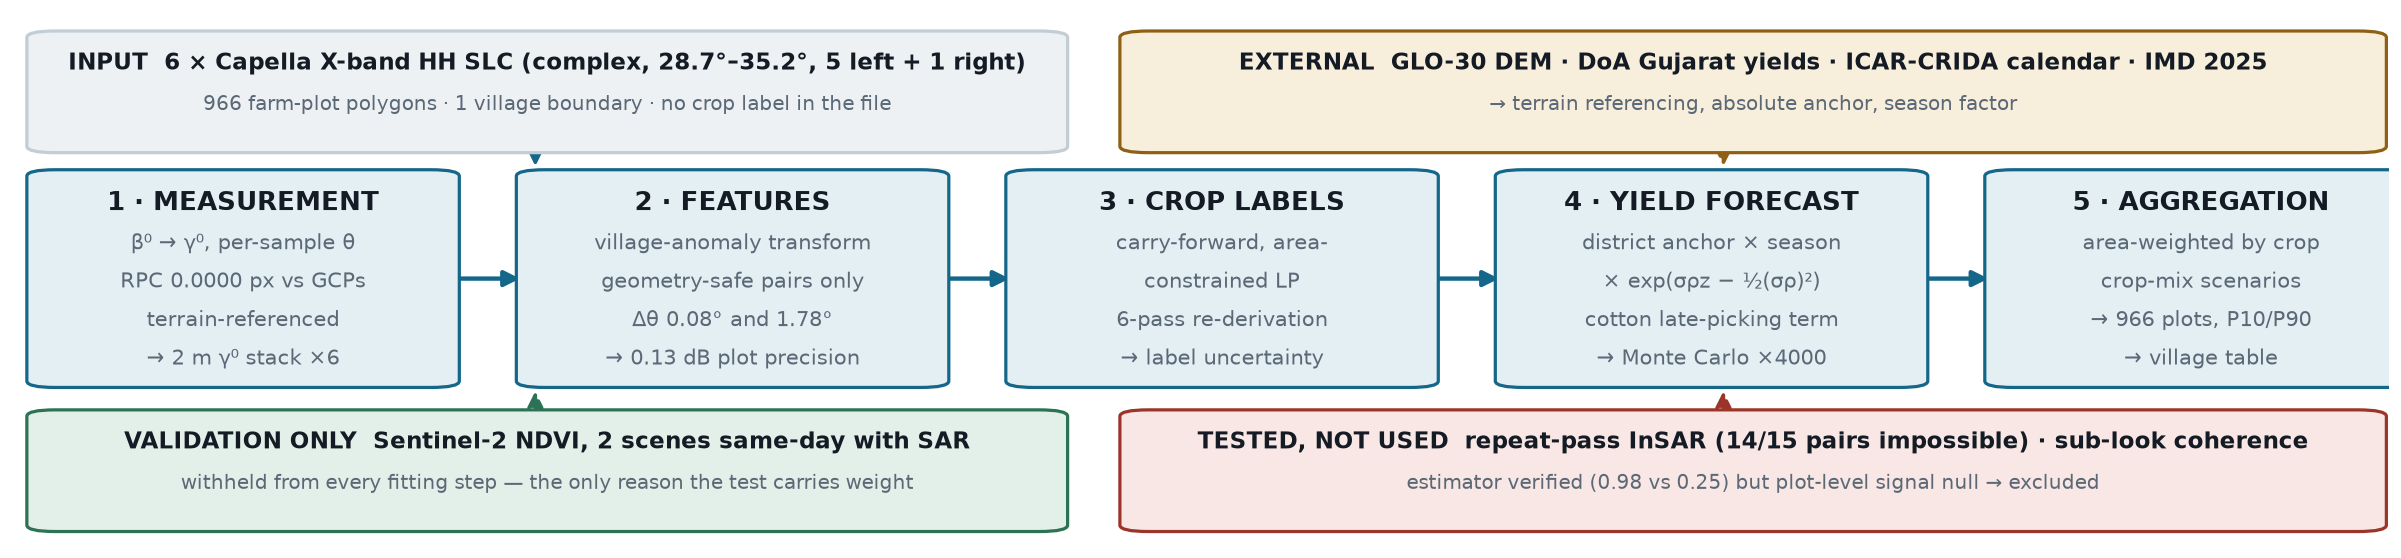
\includegraphics[width=\textwidth]{figures/architecture.png}
\vspace{4pt}
\end{minipage}\end{center}
}]

\banner{Page 1: Problem, Strategy, and Novelty}

\section{Proposed Strategy \& Technical Novelty}

\subsection{AI methodology.} This track publishes \textbf{no plot-level ground-truth yield} — not
withheld, absent. A supervised regressor has nothing to fit: an off-the-shelf regression baseline is
not weaker here, it is \emph{undefined}. Round 2 answered that with two \emph{relative} indices;
Round 3 must return \emph{absolute} kg/ha at harvest. So radar sets structure, official statistics
set level:

\vspace{-3pt}
\begin{center}
$Y_p = Y_{\text{ref}}(c)\,S(c)\,\exp\!\big(\sigma_c\rho z_p-\tfrac12(\sigma_c\rho)^2\big)$
\end{center}
\vspace{-3pt}

$z_p$ is a stage-weighted SAR index (establishment · 13 Oct canopy · 12 Nov retention · evenness);
$\sigma_c$ the farm-to-farm yield CV inside a village; $\rho$ the share of it six X-band passes
explain. Crop assignment stays an \textbf{area-constrained transportation LP} against phenological
templates — not a trained classifier.

\subsection{Novel contribution — the twist.}
\begin{itemize}
\item \textbf{The lognormal form \emph{is} the agronomic plausibility constraint.} It forces the
\emph{area-weighted} village mean to reproduce $Y_{\text{ref}}\!\cdot\!S$ \textbf{by construction},
so the level is a declared assumption and everything beneath it is SAR-driven. The model is
structurally unable to invent a village yield the radar cannot support.
\item \textbf{A second geometry-safe pair, new to Round 3.} The added passes create
13 Oct$\to$12 Nov ($\Delta\theta\,1.78^\circ$, same look) — the axis separating a crop still standing
from one already cut. Round 2 had only 19 Jun$\to$14 Aug ($0.08^\circ$).
\item \textbf{The right-looking pass as a terrain diagnostic.} A height error displaces opposite look
directions in \emph{opposite} senses, so a residual on 29 Oct alone is a terrain signature, not a
registration failure — and it caught our own regression (§4).
\item \textbf{An explicit forecast term.} Cotton alone still stands at the last pass; its final lint
carries a late-picking multiplier from that plot's own 13 Oct$\to$12 Nov retention (0.79–1.27).
\end{itemize}

\subsection{Success metrics — proving it without labels.}
\begin{itemize}
\item \textbf{A falsifiable physical prediction:} the index must correlate where a crop still stands
and go \emph{null} where it has been cut. An artefact correlates everywhere or nowhere (§3).
\item \textbf{Independent same-day optical:} two Sentinel-2 scenes are same-day coincident with
Capella passes, and NDVI enters no fitting step — the only thing making the test meaningful.
\item \textbf{Geometric self-consistency} (RPC error vs the 225 GCPs, co-registration residual,
agreement with Capella's GEO product) and \textbf{interval calibration} — village interval width must
order with how much of each crop's cycle was observed.
\end{itemize}

\section{Ancillary Grounding \& Assumptions}
\begin{itemize}
\item \textbf{Stated assumption.} SAR sets \emph{ranking and spread}; district yield $\times$ season
factor sets the \emph{level}. Sokhda is assumed not to depart from its district mean, as nothing in
the data justifies claiming otherwise. $\rho=0.55$ (varied 0.40–0.70) is assumed, not estimated — the
least-constrained parameter in the model.
\item \textbf{Datum, carried forward and extended.} Capella RPCs expect \emph{ellipsoidal} heights;
GLO-30 stores \emph{orthometric}. The offset is \emph{solved} from the 225 GCPs per product, now
across six scenes: $N=-62.02$\,m, scene-to-scene sd \textbf{0.12\,m}, agreeing with the four-scene
Round-2 solution to 0.06\,m.
\item \textbf{Known issue — swath coverage.} The AOI is wider than one Capella stripmap: 832 plots
carry all six dates, 91 partial, \textbf{43 none}. The 43 get the crop mean with inflated uncertainty
and a \texttt{not\_observed\_swath\_edge} flag — shipped, not dropped.
\item \textbf{Known issue — contaminated baseline.} Sentinel-2 shows \textbf{326 plots already green
on 10 June}, so a naive per-plot ``bare soil'' reference is itself contaminated. Features are
village-anomaly referenced instead.
\item \textbf{Known issue — label provenance.} Crop labels are the Round-1/2 carry-forward:
self-derived, not organiser ground truth, median confidence 0.16. Propagated as uncertain, not
trusted (§4).
\end{itemize}

\newpage
\banner{Page 2: Evidence, Obstacles, and Execution}

\section{Preliminary Salient Results}

\subsection{Validation note.} This track publishes \textbf{no plot-level ground-truth yield at any
stage}, so RMSE / MAE / $R^2$ and a spatially held-out split are \emph{not computable} — reporting
them would require inventing labels. We report instead (a) agreement with an \textbf{independent
sensor never used in fitting} and (b) internal geometric consistency. All 966 plots carry a forecast.

\begin{callout}{the discriminating result}
SAR yield index vs.\ \emph{same-day} Sentinel-2 NDVI (13 Oct), computed \emph{within} crop:

\vspace{2pt}
{\fontsize{7.2}{8.4}\selectfont\ttfamily
\begin{tabular}{@{}lrrl@{}}
CROP      & RHO    & P        & ON 13 OCT\\[1pt]
Rice      & +0.365 & 2e--08   & standing\\
Cotton    & +0.361 & 1e--12   & standing\\
Groundnut & +0.112 & 0.079    & harvesting\\
Maize     & +0.019 & 0.88     & harvested\\
Bajra     & --0.071 & 0.61    & harvested\\
\end{tabular}}

\vspace{2.5pt}
Significant for the two crops still in the field; \textbf{statistically null for the three already
cut}, where both sensors see bare soil. This is the §1 prediction passing. Whole village, same day:
$\rho=+0.56$ (13 Oct, $n{=}923$) and $+0.48$ (12 Nov, $n{=}937$).
\end{callout}

\subsection{Geometric progress, quantified.} RPC forward model vs.\ the 225 embedded GCPs:
\textbf{0.0000\,px}. Restoring terrain referencing improved the GCP round trip from
\textbf{15.1–16.6\,px to 4.1–4.7\,px}, raised correlation with Capella's own GEO product
\textbf{0.769\,$\to$\,0.840} on \emph{6 of 6} passes, and collapsed the right-look co-registration
residual \textbf{2.54\,m\,$\to$\,0.12\,m}.

\begin{center}
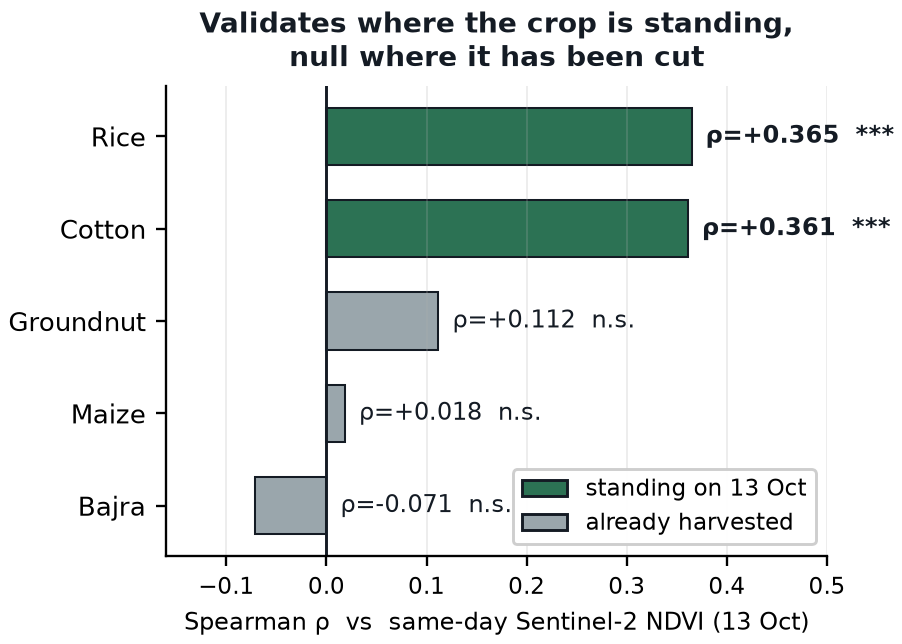
\includegraphics[width=0.995\columnwidth]{figures/validation.png}
\end{center}

\subsection{Village-level forecast.} Area-weighted, all 966 plots. Interval width orders correctly
with cycle coverage — bajra widest at $\pm$20\%, rice tightest.

\vspace{1pt}
{\fontsize{7.2}{8.6}\selectfont\ttfamily
\begin{tabular}{@{}lrrrr@{}}
CROP      & HA    & KG/HA & P10--P90     & TONNES\\[1pt]
Rice      &  60.4 &  1717 & 1401--2021   & 103.7\\
Cotton    & 192.7 &   820 &  674--\ 971  & 158.0\\
Maize     &  34.3 &  2479 & 2009--2968   &  85.0\\
Bajra     &  34.6 &  2932 & 2378--3576   & 101.4\\
Groundnut & 125.6 &  2453 & 2005--2922   & 308.1\\[1pt]
VILLAGE   & 447.5 &     — &          —   & 756.1\\
\end{tabular}}

\section{Technical Challenges \& Pivots}
\begin{itemize}
\item \textbf{No ground truth (structural).} Pivot: abandoned supervised regression outright for the
anchored hybrid, and rebuilt validation around a withheld independent sensor.
\item \textbf{A 60-day gap, 14 Aug $\to$ 13 Oct}, brackets the \emph{entire} maturity and harvest of
maize, bajra and groundnut — sampled once. Not fixable; carried as wider intervals, not hidden.
\item \textbf{Pivot — we corrected a regression in our own pipeline.} The Round-3 chain was first
rebuilt on a single constant height. All six passes agreed on it, residual ${\le}2.8$\,m, so it
looked right. It was not: a global shift metric recovers the \emph{mean} alignment and hides
spatially varying terrain, and this block carries 26.6\,m of relief $=$ up to 46\,m of ground range.
The 29 Oct right-look residual exposed it; terrain referencing — Round 2's standard — was restored
and extended to six passes.
\item \textbf{Pivot — we rejected our own new classifier.} An independent six-pass crop map agreed
with the carry-forward on only \textbf{46\%} of observed plots. On withheld Sentinel-2 the
\emph{carry-forward separated better} ($\eta^2$ 0.138 vs 0.085), so we kept it and converted the
disagreement into measured label uncertainty.
\item \textbf{Extended, still null — the phase.} Round 2 ruled out repeat-pass InSAR on four scenes;
with six, all \textbf{15 pairs} fail — 5 opposite-look (the new 29 Oct), 9 beyond the critical
baseline, and the one viable pair (B$_\perp$ 844\,m) 56 days apart. We re-ran sub-look coherence in
the \emph{azimuth} aperture rather than Round 2's range sub-bands: the estimator verifies (points
$\gamma{=}0.98$ vs 0.25 clutter) and is again null at plot level ($r{=}0.02$, $\eta^2{=}0.02$). Null
in both dimensions.
\end{itemize}

\begin{callout}{the largest open risk is not the radar}
The Round-1 carry-forward puts \textbf{groundnut at 28\% of Sokhda}; the Directorate of Agriculture
puts it at \textbf{0.35\% of the district}. Both cannot be close to right, and groundnut carries a
high per-hectare reference. Running the assignment under both area constraints moves village
production \textbf{763\,t $\to$ 570\,t ($-$25\%)}, essentially all of it groundnut. We publish both
scenarios rather than choose silently.
\end{callout}

\section{Final Sprint Roadmap}

\subsection{Immediate (next 10 hours).} Upload the executed notebook to Kaggle and set it
\textbf{public}; attach it plus the nine media-gallery figures, the written methodology and the Goa
deck; select the Track and \textbf{hit Submit} — a saved draft is not judged. Final read-through of
the 2{,}000-word writeup against the rubric.

\subsection{Refinement (running / queued).} Sensitivity of the village total to $\rho$ across
0.40–0.70; re-running the crop-mix scenarios with the district constraint as primary, to bound the
groundnut risk from both sides; rehearsing the 16-slide deck to the 10-minute limit.

\subsection{Final output.} A public end-to-end notebook (raw complex SLC $\to$ both output tables,
verified to reproduce them \emph{exactly} from a fresh kernel, closing with assertions); a
plot-level CSV of 966 forecasts with P10/P90 and quality flags; a village table by crop; a
machine-readable validation report; and the Goa presentation. \textbf{No trained model artefact — by
design, because there is nothing to train on.}

\vspace{3pt}
{\color{rule}\rule{\columnwidth}{0.5pt}}

{\fontsize{6.9}{8.2}\selectfont
\textbf{Appendix.} \textbf{GitHub:} \url{https://github.com/harshthummar77/AISEHack-2.0-ROUND-3}\;·\;
\textbf{Kaggle notebook:} public at submission, linked in the Writeup's Project Files.\;
\textbf{Data:} Capella X-band HH SLC $\times$6 (competition) · Copernicus DEM GLO-30 tile N22E073,
AWS Open Data · Sentinel-2 L2A via Element84 Earth Search, \emph{validation only} · Directorate of
Agriculture Gujarat, \emph{Area, Production and Yield} (2024) · ICAR-CRIDA/AAU-Anand, \emph{Agriculture
Contingency Plan: Vadodara} · IMD/Gujarat SEOC 2025 monsoon summary.\;
\textbf{References:} Attema \& Ulaby (1978), \emph{Vegetation modeled as a water cloud}, Radio Sci.
13(2) 357–364 · Parmar \& Bhatt (2025), \emph{Agricultural patterns and crop shifts in
Vadodara-Chhotaudepur}, IJAFS 7(5) 55–61 · Monteith (1977), radiation-use efficiency · Capella Space,
\emph{SAR Imagery Products Format Specification} (radiometry, RPC, NESZ).}

\end{document}
